\chapter{绪论}

\textbf{本章摘要:} 本章首先介绍了网络经济学的背景、网络外部性效应的基本概念及其在移动网络中的体现; 
接着分析总结了近些年国内外涉及到激励机制设计、隐私保护等与本文中网络性能优化场景相关领域的研究现状;
最后阐述了本文的研究思路和研究内容。

\textbf{关键词:} 网络经济学;网络外部性;机制设计;隐私保护;群智感知;研究背景;研究现状

%\keywords{毫米波通信;5G;资源优化}

\section{研究背景}
%当今世界是一个网络的世界,各种形式的网络在人们生活中随处可见、无处不在。例如,由移动设备作为节点,由通信链路连接而成的移动通信网;社交网络是由每个人作为节点,每条边由人们之间的社交关系定义;电力网络则是由包含了发电站、配电站、工厂、办公楼、电动车充电站等电力设施以及它们之间的电力传输线路所组成的网络;而交通运输网络则是由各个运输枢纽以及连接他们的运输线路、运输工具所定义的。这些客观存在的以及人们创造出来的网络充斥着整个社会和我们的生活。

当今世界是一个网络的世界,各种形式的网络在人们生活中随处可见、无处不在。这其中包括,由移动通信设备作为节点、通信链路连接而成的移动通信网,节点对应每个人、连边代表人与人之间社交联系的社交网络,由发电站、配电站、工厂、办公楼、电动车充电站这些电力设施以及它们之间的电力传输线路所组成的电力网络,以及由各个运输枢纽与连接他们的运输线路、运输工具所定义的交通运输网络。在本研究中,我们所关注的主要对象是移动通信网络,同时也涉及到由移动网络中用户之间社交联系所定义的社交网络。

\subsection{移动网络中的网络经济学}

移动通信网络具有两个显著的特征。首先,相对于不断增长的用户数量以及流量需求,移动通信网络普遍存在资源有限甚至缺乏的特性。其具体表现在每一个移动设备上的通信、计算、能耗等资源都是有限的,此外移动无线通信所能使用的频谱资源是有限的,通信总带宽是一定的。由此,通信运营商始终面临的一个难题即是如何高效、公平地对带宽进行分配,使用户在通信过程中受到的信号干扰控制在可接受的范围内,实现尽可能高的通信质量保证。移动通信网络的另一个特征则是网络中的个体相对独立,且具有自利属性。这些个体大到不同的网络运营商(例如中国移动、中国联通),小到终端的一个移动设备(例如智能手机),都是以最大化自身利益为目标的。这种情况下,网络系统的全局最优解通常是难以达到的,而实现网络性能的提升与优化则依赖于个体之间在有效的激励机制作用下的协同合作。  

上述的两个特征使得移动通信网络中的很多性能优化问题具有明显的经济学特征。针对资源有限的特性,网络效用最大化(Network utility maximization)的一系列理论工具已经在对于诸如网络吞吐量、延迟、公平性等指标的优化研究中取得了显著的成果\cite{NET}。而针对网络中用户的个体自利属性,则更多需要借助网络经济学中的一些概念工具对相关问题进行建模求解。包括“非合作博弈”、“拍卖理论”、“纳什均衡”在内的一系列经济学概念原理\cite{osborne}已经被广泛应用于各种移动通信网络中的资源分配与系统优化问题中。在一些问题背景下,移动用户的集合、他们对应的行为策略集合以及他们各自效用函数的集合即可构成一个典型的博弈模型。在博弈模型中,每个用户作为玩家以最大化自身的效用为目标,针对其他用户的策略做出最优相应(Best response)。当博弈处于其均衡状态时,给定其他用户的决策,任何用户都无法通过单独改变自己的决策以获得个体效用的提升。然而,从网络整体的角度来看,博弈均衡状态下的系统性能可能较全局优化得到的系统性能有所损失。这种损失正是由于网络中个体的自利属性以及他们决策间的关联性所导致的。

%以移动通信网络中的数据服务定价问题为例,该问题中作为买方的移动用户购买使用服务提供商的数据流量。作为卖方的服务提供商需要考虑如何优化其定价策略以最大化其收益。该问题本质上即是一个市场交易模型下的商品定价问题,可以被建模成纳什博弈问题进行分析。


\subsubsection{网络外部性效应}

网络外部性作为网络经济学的主要研究对象之一,描述了存在于网络中个体之间相互影响的一种现象。其概念最早由Rolfs于1974年提出的\cite{Rolfs},之后Katz和Shapiro在1985年完成了正式的定义\cite{Katz}。在经济学中,网络外部性通常指某物品的一个用户给该物品对于其他用户的价值带来的影响。在本文中,网络外部性则更具一般性地指任一网络参与者受到网络中其他参与者非直接影响所导致其效用(Utility)上的损失或受益。这种影响可能简单取决于其他参与者的数量,也就是网络的规模,同时也可能取决于网络中个体的参与程度或者个体之间的关联强度\cite{externality}。

%这时网络外部性通常也被称为网络效应。比如,在一个有线电话网络中,如果参与这个网络的用户越多,每一个用户可能从这个网络中获得的好处越大,因为用户可以使用电话或传真来联络的用户会越多,通信交流更加方便。每一个新增的用户,都给所有现存的用户增加了潜在的联系对象,因此也会提高所有老用户的效用。
%除了网络规模的影响外,网络外部性在一些更为复杂的情况下还体现为参与者的参与程度对每一个独立个体的影响。
依据不同的分析视角,网络外部性现象可以被进一步细分。常见的划分方式将网络外部性分为正网络外部性与负网络外部性两类。简单来说,如果用户所获得的效用随其他用户参与程度增加而增加,则为正网络外部性,相反若用户效用随其他用户参与程度增加而降低则为负网络外部性。典型的正网络外部性的例子包括电话网络,使用电话进行联络的用户数量越多,则对于每一个使用电话的用户其效用越大。负网络外部性现象\cite{negative}也较为普遍的存在于生活中的很多场景中,例如机动车辆数量增多带来的交通拥堵,化工企业数量增多带来的空气污染、水污染等。网络外部性的其他分类方式还包括直接网络外部性或间接网络外部性、单边网络外部性或双边网络外部性等。此外,当个体只受到网络中一部分用户的影响时,网络外部性还可以被定义为一种{\kaishu 局部网络影响},例如社交网络影响\cite{jianweibook}。
%	\item \textbf{单边网络效应/双边网络效应} 单边效应是指产生于单边网络中同类用户之间的网络效应。而在一个双边网络里,两类不同的用户之间会产生跨边的网络效应,即网络一边参与用户的效用会受到网络另一边参与用户的影响。例如阿里巴巴的支付宝服务,接受支付宝付款的商户越多,支付宝用户就会享受到越多的支付便利。反过来,支付宝用户越多,接受支付宝付款的商户就可能获得更多的商机。另一个例子比如操作系统与其兼容的软件。


%近些年,移动通信技术的飞速发展推动了移动社交网络与相关应用的普及与流行。例如包括微信、QQ在内的基于社交的即时通信应用大大促进了人们的在线社交活动,改变了人们的交流沟通方式,同时也对人们的数据流量使用行为产生了影响。
%例如基于社交网络的在线游戏应用,通常用户的效用体验是随着其在线好友数量增多而增加的。对于一个移动用户,如果其社交好友都热衷于某一手机游戏,那么该用户很有可能也会成为该游戏的玩家。
%这种社交影响最终会导致用户更多的数据流量使用。这种现象即是我们所要讨论的网络外部性的一种典型的体现。

近年来,移动通信技术的飞速发展、移动设备的普及、网络规模的不断扩大、以及移动社交应用的盛行,使得一些移动网络问题中的网络外部性现象愈发凸显出来。而在对这些问题的分析建模过程中考虑网络外部性的影响则具有十分重要的意义。
%当一个移动网络场景中存在网络外部性现象时,在建模过程中充分将网络外部性的影响考虑进去将有利于网络设计的优化,有效提升网络中个体效用以及网络的整体性能。
例如在网络服务定价问题中,作为一个服务提供商,如果其掌握了移动用户的社交关联信息,那么其可以在考虑社交影响带来的正网络外部性的基础上,进行定价策略的优化。在这种情况下,使用无线数据服务给用户带来的价值可以被分成两部分,一部分是用户自身使用服务获得的效用,另一部分是与其有社交关联的用户同时使用服务所带来的额外效用。因此,如果提供商在优化定价策略时仅考虑前者而忽略了后者则可能使得到的收益偏离实际可达到的最优收益。相反如果提供商适当降低服务价格以吸引更多用户的参与,则用户在正网络外部性影响下可获得更多的效用,进而使用更多的数据服务,给服务提供商带来额外的收益。

\subsubsection{理性行为模型}
在移动网络中,通常假设通信或数据资源的持有者和使用者为独立的个体,他们了解自己可以选择的决策,对于所得到的不同的结果有明确的偏好。这些独立个体执行最大化个人效用的行为则被称之为理性(Rational)行为。而个体信息的不完整以及不确定性,甚至个体对自身或他人策略的非客观性评估,会使得实际中个体行为偏离理性行为,其被称之为有限理性(Bounded-rational)行为。行为经济学(Behavioral Economics)对于个体的非完全理性行为有着广泛且深入的研究,其中就包括获得2002年诺贝尔奖经济学奖的展望理论(Prospect Theory)\cite{Kahneman}。在具有不确定性的环境中,相比于通常用于求解最优策略所使用的期望效用理论(Expected Utility Theory),展望理论提供了对于决策制定在行为心理学上更加准确的描述,从相关实验研究的结果上看其更加贴近真实中的情况。在移动网络的一些问题场景中,展望理论有着较大的应用价值。在移动网络中的机制设计中,充分的考虑不同用户行为模型上的异质性是至关重要的。

\subsection{移动网络性能优化机制设计}
借助于网络经济学的理论工具,人们可以通过对移动网络运作机制的巧妙设计实现对于复杂网络系统建立更加实际的模型并进行求解。下面我们对本文所涉及的三个移动网络机制设计问题进行简单的介绍:
\begin{itemize}
\item \textbf{分布式频谱接入机制:} 移动通信网络中所使用的的频谱是一种典型的稀缺资源,当空间上临近的两个通信链路同时使用同一频段时会互相产生干扰,影响通信的质量。在这种情况下,有限的频谱带宽中又有大部分被划分为只有“主用户”可以使用的专用频段。动态频谱共享技术的出现大大改善了频谱的使用效率,使得无频谱使用执照的移动设备可以以“次级用户”的身份机会性地在“主用户”未使用其频段时接入频段,被认为是解决频谱利用问题的有效解决方案。然而在规模较大的移动网络场景中,由于个体用户普遍具有自利属性,如何为大量次级用户设计高效的分布式频谱共享接入机制以优化系统的整体性能仍然面临着较大的挑战。较为常见的一类解决方案是将次级用户之间的交互建模成非合作博弈\cite{wang2010game, chen2012spatial}。


\item \textbf{数据服务定价机制:} 一个移动通信网络是由网络运营商(数据服务提供商)和众多移动用户(数据服务使用者)所组成的。运营商制定数据服务的价格,而用户基于观察到的价格决定自己的数据使用需求量。对于数据服务定价机制的研究需要将对于用户行为的分析与对于运营商价格策略的优化有效地结合起来。价格策略是运营商追求收益优化的重要杠杆。较高的价格在得到更大边际收益的同时可能会抑制用户的需求,而较低的价格有助于扩大其用户市场,而会造成一定的收益损失。在对用户行为的建模中,当假设其决策不考虑自身数据使用行为对于价格的潜在影响时,这些用户被称为价格接受者(price-taker)。相反,当假设用户的决策考虑了网络中其他用户的行为及其影响时,这些用户被称为价格预期者(price-anticipator),此时对于用户的行为策略的建模和分析需借助博弈论的理论工具。价格预期者类型的用户、多个运营商之间的竞争以及服务市场供需两侧的信息不完整都会给数据服务定价机制的设计带来不小的挑战。

\item \textbf{群智感知激励机制:} 群智感知基于众包的思想,将感知任务指派给移动设备来完成,并支付给移动用户一定奖励以补偿用户的资源消耗。与频谱选择和数据服务消费场景所不同,群智感知中的感知、计算资源属于移动用户,系统则需要通过有效的激励机制向用户提供激励,鼓励用户参与并贡献其感知资源。在一些场景中,为了对用户资源进行协调调度,系统需向用户获取一些有关用户资源的信息(例如移动用户的感知成本、数据隐私偏好等)。而对于激励机制设计的一个主要挑战即是如何促使用户诚实地提供所需的个人相关信息。常见的用于群智感知激励机制设计包括基于反向拍卖模型的机制\cite{yang2012crowdsourcing},具体包括确定拍卖赢家(Winner-determination)和确定相应的奖励金额(Price-determination)两步。此外,如何消除用户对于贡献个人数据所产生的隐私顾虑也已成为相关研究关注的重点。
\end{itemize}

%\subsection{移动网络中的隐私保护}
%由于移动设备与用户的强关联性,移动网络中的隐私保护问题早已成为国内外社会所共同关注的焦点问题。近年来,由于隐私保护措施不力导致的严重隐私泄露事件时有发生


\section{研究现状}

\subsection{移动网络中的网络外部性效应}
%在这一小节,我们结合一些移动网络中的具体场景,对移动网络中涉及到网络外部性效应的一些现有研究进行介绍。

%我们首先简要回顾一下有关具有社交意识的频谱共享的相关工作。Li等\cite{li2011propagation}对认知无线电网络中的社交行为进行了社交网络上的分析。另一种常见的基于社交互动的频谱共享模型是将次级用户具有利己性质的行为互动建模为非合作博弈\cite{wang2010game}。

随着越来越多的移动用户通过在线社交网络(例如Facebook \cite{FB},Twitter\cite{Twitter})进行联络,用户的影响力和信息传播速度已经达到了前所未有的速度\cite{Niyato}。作为一种典型的局部网络外部性效应,移动网络的社交影响引起了服务提供商以及平台开发人员的广泛关注。David等\cite{David10}将用户之间的社交效应建模为一种正网络外部性效应。Chen等\cite{Baochun}采用了类似的想法来刻画众包系统中不断增长的社交用户数量所带来的内在收益的增长,及其对于平台外在奖励开支的削减。为了减少蜂窝网络峰值负载,Malandrino等\cite{social}提出了一系列算法,根据用户在社交网络中的地位将数据内容主动地推送给一些特定用户。一些研究工作已经在解决网络设计和优化问题中对于个体间的社交影响进行充分的考量。Chen等\cite{Chen13}利用社交信任和互惠互利因素,通过将问题转化为联合博弈来改进D2D合作通信质量。Li等\cite{li2011propagation}针对认知无线电网络中个体的社交行为进行了社交网络分析。Ashraf等\cite{Ashraf}使用用户之间的社交距离确定用户关联,基于此实现了具有底层D2D通信的小型蜂窝网络系统性能上的提升。Yang等\cite{Guang}提出了一种移动群智感知系统设计,利用移动用户之间的社交联系来激励他们的参与和合作,以获取更高的回报。Chen等\cite{Chen14}提出了一个社交群体效用最大化(SGUM)框架,其中每个用户以自己的个人效用与社交朋友的效用所组成的“群体效用”为优化目标。

%在移动频谱共享机制的研究领域,近年来的一些以优化系统效用为目标的研究工作都考虑了用户间的社交影响。Li等\cite{li2011propagation}针对认知无线电网络中个体的社交行为进行了社交网络分析。另一种

%We start with a brief review on related work on socially-aware spectrum sharing. Xing \emph{et al.}~proposed to use anthropological models in human society to enhance the performance of cognitive radio networks \cite{xing2008human}. Li \emph{et al.} \cite{li2011propagation} carried out social network analysis of the social behavior in cognitive radio networks. Another common approach for spectrum sharing based on social interactions is to model secondary users' interactions as noncooperative game (e.g., \cite{wang2010game} and many others) assuming they are \emph{selfish yet rational}. Notably, Chen \emph{et al.} \cite{chen2012spatial} developed a spatial spectrum access game framework to model the competitive spectrum access among the secondary users by taking the spatial reuse effect into account. 
%\subsubsection{移动网络中的负网络外部性}
除了社交效应所导致的正网络外部性效应,负网络外部性现象也存在于很多移动网络问题场景中。例如,在通信网络中,当用户数量增加使得流量负载超出基础架构容量时,就会发生拥塞现象。
%拥塞效应在一些数据速率较低的通信场景(例如\cite{Jiming}和\cite{Deng})中的影响可能并不突出,然而其在
这种影响在许多数据通信速率较高的移动网络系统中尤为显著,目前已有相关工作对其进行了深入的研究\cite{Asuman07,Fang09,Tran12,rayliu2,rayliu3}。其中Yang等\cite{rayliu2}使用随机博弈模型对无线接入网络选择问题进行建模,并充分考虑了不同用户选择同一无线网络所导致的拥塞效应。移动网络中的另一种常见的负网络外部性现象是移动设备间的信号干扰。接入一个信道的用户越多,每个用户所可以获得的吞吐量越低。因而当移动设备在做信道接入决策时,除了考虑信道的通信质量,还需考虑其他设备的信道接入选择。Jiang等\cite{rayliu1}在研究多信道感知接入的问题时就从网络外部性的角度将信号干扰作为影响次级用户顺序信道接入决策的主要因素并进行相关分析。
%\subsubsection{Ray Liu}
%负网络外部性

\iffalse
\subsection{移动无线网络机制设计}
\subsubsection{群智感知激励机制}
移动群智感知系统的激励机制设计最近受到了广泛关注\cite{yang2012crowdsourcing,feng2014trac,Zhao,wen2015quality,zhang2015incentivize,zhang2015truthful,jin2015quality,jin2016inception,zhang2016privacy,duan2012incentive,Shibo14,peng2015pay,cheung2015distributed,he2017exchange}。不同的模型例如拍卖模型\cite{yang2012crowdsourcing,feng2014trac,Zhao,wen2015quality,zhang2015incentivize,zhang2015truthful,jin2015quality,jin2016inception,zhang2016privacy}和博弈模型\cite{duan2012incentive,Shibo14,peng2015pay,cheung2015distributed,he2017exchange}已经被用于设计具有不同目标的激励机制,其中包括社会福利最大化\cite{cheung2015distributed,gao2015providing,jin2015quality},成本或付款最小化\cite{feng2014trac,jin2016inception}以及平台的利润最大化\cite{Shibo14,zhang2016privacy}。然而现有的大多数工作\cite{yang2012crowdsourcing,feng2014trac,Zhao,wen2015quality,zhang2015incentivize,zhang2015truthful,jin2015quality}仅考虑了参与者的感知成本。

\subsubsection{无线数据定价机制}
通信网络中的定价问题已经在文献\cite{Walrand08,Huang10,Xinbin,CaoTVT,Xiaoming}中得到了较好的解决。在一些重点关注单个服务提供商定价策略的研究工作中,移动用户的数据使用行为所受到正面网络影响已经被考虑进来,如\cite{Hartline08,Candogan12,SwapnaES12}。而据我们所知,目前还很少有在研究网络服务定价问题中同时考虑到网络效应和拥塞效应的影响。最近,Gong等\cite{GongDCZ17}首先研究了垄断市场中单个服务提供商的定价策略,在该市场中,移动用户的数据使用行为会同时受到这两种影响。相比于上述工作中所考虑的垄断市场,我们的前期工作\cite{MYCISS16}研究了寡头市场环境下的定价问题,即存在多个服务提供商之间争夺移动用户的数据市场的竞争。
\fi

\iffalse
\subsection{差分隐私保护}
本小节将介绍差分隐私的一些基本知识。我们从介绍

\subsubsection{贝叶斯隐私攻击模型} 
我们假设一个移动用户的隐私数据字段为$x\in\ca{X}$,其中$\ca{X}$代表数据取值的区间。我们同时假设攻击者攻击者具有针对目标用户数据字段$x\in\ca{X}$的分布$\pi(x)$的{\kaishu 先验}知识,以及数据$x\in\ca{X}$被模糊为$x^*\in\ca{X}$的概率$p(x^*|x)$。则攻击者根据贝叶斯规则以及观察值$x^*$可以推断出目标用户真实数据取值的{\kaishu 后验}分布$p(x|x^*)$:
%We assume that a mobile user has private sensing data $x\in\ca{X}$ with $\ca{X}$ denoting the domain of the data value. We also assume that an adversary has the \emph{prior} knowledge about the probabilistic distribution $\pi(x)$ of a participated user's sensing result $x\in\ca{X}$, as well as the probability $p(x^*|x)$ under which a sensing data $x\in\ca{X}$ is obfuscated to $x^*\in\ca{X}$. Then, with the observation of $x^*$, the attacker can derive a \emph{posterior} distribution of user's true sensing result, $p(x|x^*)$, based on Bayes' rule\cite{Leye}:
\begin{equation}
p(x|x^*)=\frac{p(x^*|x)\cdot\pi(x)}{\sum_{x'\in\ca{X}}p(x^*|x')\cdot\pi(x')}.
\end{equation}
在应对这种贝叶斯隐私攻击时,有效的机制应当可以限制攻击者后验知识较其先验知识的提高。换句话说,若$p(x^*|x)$和$p(x^*|x')$足够接近到对于攻击者来说,观察到$x^*$并不能帮助其有效地区分$x$和$x'$,则说明防御机制是有效的。
%In order to combat this Bayesian privacy attack, we design a privacy-preserving mechanism that can bound the improvement of the attacker's \emph{posterior} knowledge over her \emph{prior} knowledge. In other words, it is desirable to have the value of $p(x^*|x)$ and $p(x^*|x')$ close enough so that, given the observation $x^*$, the attacker can hardly distinguish $x$ and $x'$. To this end, we resort to the celebrated notion of differential privacy.

\subsubsection{差分隐私} 
根据\cite{wang2016value}, 我们定义一个用户的差分隐私保护级别如下。
\begin{df}[差分隐私保护级别]\label{def1}
用户的差分隐私保护级别$\epsilon$定义如下
\begin{equation}
\epsilon = \max\left\{\ln\left(\frac{p(x^*|x)}{p(x^*|x')}\right)\right\}, ~\forall x, x'\in\ca{X}.
\end{equation}
\end{df}
用户的$ DPL $通过测量报告数据的条件概率之间的可分辨性,量化了攻击者在\\ emph {pri}知识下的潜在隐私泄漏。可以容易地证明,在$ DPL = \ epsilon $的情况下,攻击者的知识增益$ g = p(x | x ^ *)/ p(x)$被限制为$ 1 / e ^ \ epsilon \ leq g \ leq e ^ \ epsilon $和\ emph {先前}的知识$ p(x)$。显然,\ epsilon $越小,攻击者就越难正确地推断出真实数据,因此,保护​​隐私的性能就越好。接下来,我们回顾两种本地数据扰动方法,通过这种方法,可以为用户数据实现一定的差异性隐私保护级别。
%A user's $DPL$ quantifies the potential leakage of privacy under the \emph{prior} knowledge of attacker by measuring the indistinguishability between the conditional probability of the reported data. It can be easily proved that with $DPL=\epsilon$, the knowledge gain of an attacker, $g=p(x|x^*)/p(x)$, is bounded as $1/e^\epsilon\leq g\leq e^\epsilon$ with \emph{prior} knowledge $p(x)$. Clearly, the smaller the $\epsilon$, the harder for the attacker to correctly infer out the true data, and hence the better the privacy-preserving performance. We next review two local data perturbation methods, by which a certain differential privacy-preserving level for a user's data can be achieved.

\subsubsection{差分隐私机制}
\textbf{拉普拉斯机制.}
Laplace mechanism is a widely used technique that provides differential privacy gurantees\cite{dwork2014algorithmic}. In this paper, we are interested especially in a variant version of Laplace mechanism, in which a Laplacian noise $\eta\sim Lap(\Delta/\epsilon)$ is added locally to each individual user's data where $\Delta \triangleq \max_{x,x'\in\ca{X}}|x-x'|$ is defined as the local sensitivity and $\epsilon$ is the $DPL$ of that user.  

\textbf{随机回应机制.}
Randomized response is another tool that can provide local differential privacy guarantees\cite{dwork2014algorithmic}. With certain probability, the individual user sends a random instance of her real data to the untrusted data collector. The parameters of randomized response mechanism are carefully chosen to limit the platform's ability to learn with confidence about the true value of the data. %As an illustrating example, when the data is one bit binary data, the data owner can flip a biased coin, and report the truth to the platform if the coin comes up head, and tell the opposite answer if it comes up tail. The data owner thus preserves the data privacy due to the coin randomness.
\fi


%\subsection{移动无线保隐私机制设计}
\subsection{群智感知系统中的数据隐私保护}
在群智感知系统中,用户在向感知平台提供数据的过程中往往会直接或者间接地泄露与用户相关的敏感信息。因次,参与用户在产生感知成本的同时也会付出一定隐私成本。
近些年,研究者们开始对群智感知系统中的数据隐私保护给予更多的关注\cite{christin2011survey,dandekar2014privacy,ghosh2015selling,jin2016inception,zhang2016privacy,wang2016value,gong2017truthful}。其中大多数工作\cite{christin2011survey,dandekar2014privacy,ghosh2015selling,jin2016inception,zhang2016privacy}在建模中假定群智感知平台是值得信赖的,用户直接将原始感知数据发送给作为数据收集方的感知平台,将数据隐私保护控制权完全交给了感知平台。近期的工作\cite{wang2016value,wang2016buying}更多考虑了感知平台为非可信的情况,并允许用户通过报告含有噪声的数据来对其隐私进行保护。本小节将介绍几种与本文相关的移动群智感知隐私保护设计,这些设计将基于差分隐私的数据加噪与激励机制设计相结合,把对于用户隐私成本的补偿考虑到激励机制的设计中。下文根据所使用的激励机制的类型对相关工作进行分类,包括基于{\kaishu 拍卖模型}的方法,基于{\kaishu 博弈模型}的方法和基于{\kaishu 合约模型}的方法。

%\rv{并在博弈论模型框架下把隐私数据作为可交易的私人商品,然而}


%In this section, we give an overview of several state-of-art privacy-preserving MCS designs that integrate differential-private noise injection with incentive mechanism design. We classify these works according to the types of incentive mechanisms they used, which includes \emph{auction} based approach, \emph{game theory} based approach, and \emph{contract theory} based approach.



%\subsubsection{基于拍卖模型的方法}
%The (reverse) auction mechanism is one of the most popular approaches for platform-centric MCS incentive mechanism design. In specific, the platform acts as the auctioneer and the mobile users report their bids reflecting their participation costs to the platform. The platform selects the participants and determines the corresponding payments, aiming to minimize the total payment or to maximize the platform utility under the budget constraint, or to maximize the participants' social welfare\cite{DejunJ}. 

\noindent\textbf{基于拍卖模型的方法:}反向拍卖机制是移动群智感知系统常用的激励机制类型之一。具体来说,由平台充当拍卖商移动用户向平台报告其出价,反映其参与成本。该平台选择参与者并确定相应的付款,目的是在预算约束下使总付款最小化或使平台效用最大化,或使参与者的社会福利最大化\cite{DejunJ}。Ghosh和Roth的工作\cite{ghosh2015selling}首创性地提出了一种可用于保护用户数据隐私的拍卖机制,其中用户的出价反映了其单位隐私成本,并令用户单位隐私成本与差分隐私保护级别$\epsilon$的乘积来刻画用户的隐私损失。文中所设计的拍卖机制满足激励机制设计的两个基本要求,即诚实性(Truthfulness)和个体合理性(Individual Rationality):
%In the seminar work by Ghosh and Roth \cite{ghosh2015selling}, an auction mechanism was proposed, where the private data is treated as goods procured by a data analyzer running a survey. Each individual's privacy cost is modeled as a linear function of her differential-privacy-preserving level $\epsilon$. The designed auction mechanism satisfies two fundamental requirements for incentive mechanism design, i.e., truthfulness and individual rationality:
\begin{itemize}
%\item Truthfulness: A participated user cannot benefit from bidding untruthfully.
\item \textbf{诚实性}:参与用户无法通过不诚实的出价行为获取收益上的提升。
%\item Individual Rationality: Each participated user receives a payment that is larger than or equal to her privacy cost.
\item \textbf{个体合理性}:每个参与用户收到的奖励不低于其隐私损失。
\end{itemize}
%This work\cite{ghosh2015selling} characterizes the tradeoff between the total payment and the result accuracy from the following two perspectives: 1) to minimize the total payment given an accuracy requirement, or 2) to maximize the result accuracy under a payment budget. 
Ghosh等\cite{ghosh2015selling}从以下两个角度描述了数据收集者付给用户的总奖励额与数据聚合结果准确性之间的折衷:(1)在给定准确性要求的情况下最小化总奖励额;(2)在给定总奖励额预算情况下最大化数据聚合结果准确性。在此基础上,Jin等\cite{jin2016inception}开发了一个用于在移动群智感知系统中保护用户数据隐私的组合拍卖机制框架。除了在建模中将隐私成本作为用户感知成本的一部分,作者在解决用户选择问题中还考虑了感知用户可靠性对聚合结果准确性的影响。另一相关工作[\citenum{zhang2016privacy}]则考虑了移动用户行为受社交因素的影响。值得注意的是,以上工作在建模过程中都假设数据收集者为可信第三方。
%Along this line, Jin \textsl{et al.} developed a combinatorial auction based framework for preserving data privacy in MCS \cite{jin2016}. Specifically, the privacy cost is modeled as part of each user's sensing cost. In addition, the reliability of mobile users, which influences the accuracy of aggregated sensing results, is further considered during the user selection. Related works \cite{zhang2016privacy} considered a setting where the mobile users are embedded in a social network. Worth noting is that both assumed a trusted data collector in their models.

% In addition, they also considered the case of real-time data aggregation in which their proposed mechanism provides long-term incentives aiming to maintain continuous participation. 
%Although the above mentioned works posses some differences in the models they used, all of them apply the Laplacian mechanism for data perturbation. 

%\subsubsection{基于博弈模型的方法}
%The game theoretic model is another popular approach for incentive mechanism design \cite{DejunJ, he2017exchange,Yang17}. 
\noindent\textbf{基于博弈模型的方法:}使用基于博弈论模型的问题建模\cite{DejunJ, he2017exchange,Yang17}是网络经济学中研究激励机制的另一种典型方法。
%As a user-centric approach, game theory based approach enables mobile users more involvements into the payment determination process. 
与基于拍卖的激励机制设计相似,基于博弈论模型的方法需要指定一种支付策略以激励用户的参与。所不同的是,在基于博弈的方法中,用户是否参与不由平台选择确定,而是用户根据平台的奖励规则做出策略性的决策。
%Similar to the auction based mechanism design, game-theoretic approaches need to specify a payment policy that incentives users' participation. However, in game based approaches, the participated users are not selected by the platform; instead, given the payment policy of the platform, users make strategic participation decisions. 
Wang等\cite{wang2016value}在一种特定背景下设计了一种博弈机制,其中数据收集者购得的用户私人数据为用户对于系统状态的认知。不同于文献[\citenum{ghosh2015selling,jin2016inception,zhang2016privacy}]中所考虑的可信平台对聚合后数据进行中心式数据加噪,Wang等\cite{wang2016value}使用了数据收集者不可信的假设。在这种前提下,每个参与用户策略性地对于其原始数据进行扰动,随后将带噪声的数据发送给数据收集者。在博弈模型中,用户为玩家其行动对应于其数据扰动策略。通过对于数据收集者定价策略的精心设计,该机制可以实现当博弈达到纳什均衡时,参与用户的隐私成本得到补偿且数据聚合结果满足一定的准确性要求。然而使用博弈论建模的方法可能会导致系统处于效率较低的均衡状态,使得数据聚合结果难以达到较高的准确性标准。
%Wang \textsl{et al.} in \cite{wang2016value} devised a game-theoretic mechanism in a setting where a data collector purchases users' private data which represents their knowledge about an underlying system state. Different from \cite{ghosh2015selling,jin2016,zhang2016privacy} where a trusted platform carries out centralized data perturbation over aggregated data, an underlying assumption in \cite{wang2016value} is that the data collector is not trustworthy, in which case each participated user is allowed to locally perturb her raw data strategically before releasing it to the data collector. In their game theoretic model, individual users are the players of the game whose actions correspond to their data perturbation strategies. And the pricing strategy is carefully designed by the data collector, so that a Nash equilibrium of the game can be achieved with participated users' privacy cost being compensated and the accuracy requirement of the collected data being satisfied.

%\subsubsection{基于合约模型的方法}
\noindent\textbf{基于契约模型的方法:}在基于契约的机制中,契约设计者将精心设计一组付出-报酬的对应选项,以激励具有不同类型的个体的参与,同时优化设计者自身的收益。基于契约的方法不要求实时的竞标信息,而是利用个体成本的统计信息来确定报酬契约,从而克服了信息不对称的问题并减少了通信和计算开销。Zhang等\cite{Kun1}提出了一种基于契约的移动群智感知隐私保护框架。具体来说,感知平台设计并公布其契约选项,每个选项都指定一种类型的查分隐私保护级别,以及用户在同意该契约选项后所可收到的相应报酬。此后,每个用户选择使自己效用最大化的契约选项之一。作者选取了适当的指标并得出了个人隐私保护级别与数据聚合准确性之间的定量关系。
%In a contract-based mechanism, the contract designer would sophistically design a menu of effort-payment pairs to incentivize the participation of individuals with different types, while at the same time optimize its own payoff. Instead of requiring real-time bid information, contract-based approach exploits the statistical information of individuals' costs to determine payment contracts, which overcomes the information asymmetry and reduces communication and computation overhead. In \cite{Kun1}, a contract-based privacy-preserving MCS framework was proposed. Specifically, the platform designs and broadcasts a menu of contracts, each of which specifies one type of differential-privacy-preserving level and the corresponding payment that a user will receive if she agrees with that contract. Each user then chooses one of the contracts that maximizes her utility. The authors derived the quantitative relationship between individual privacy and aggregation accuracy with proper metrics. 
表\ref{table:comparison}总结对上面所介绍的三类方法进行了对比。
%The three approaches reviewed above are summarized in Table 1. Although they applied different mechanism design approaches, their is one common thread: the $DPL$ of each individual user remains unchanged throughout the crowdsensing procedure. In the next section, we extend the current scenario to a more general one, in which case the mobile users' $DPL$s are not static and the platform needs to dynamically adjust the pricing policy to optiize the operation of the MCS system.

\begin{table}[!htp]
	%\caption{Summary of existing data privacy-preserving approaches for mobile crowdsensing}
	\caption{针对现有移动群智感知数据保隐私方法类型的总结}
	\centering
	\tabcolsep=10pt
	\begin{tabular}[c]{|c|c|c|c|c|}
		\hline \label{table:comparison}
		\textbf{文献} & \textbf{激励机制类型} & \textbf{平台可信} &  \textbf{数据扰动机制} & \textbf{特征} \\ \hline
		
		\cite{jin2016inception}  & 拍卖  &   是  &	拉普拉斯机制 & 考虑用户可靠性 \\ \hline

%		\cite{Kun1}	  & Auction	       &        No  	  & Laplace mechanism & Provide long-term incentive mechanism 	\\ \hline
		
		\cite{zhang2016privacy}  & 拍卖  &   是  & 拉普拉斯机制  & 考虑用户社交联系 \\ \hline

		\cite{wang2016value}  & 博弈 &    否   &   随机回应 & 分析了用户的均衡行为	\\ \hline

		\cite{Kun1}  & 契约  & 否  & 拉普拉斯机制 & 解决信息不对称问题 \\ \hline

	\end{tabular}
\end{table}


\subsection{频谱共享中的位置隐私保护}

无线网络中的另一种常见隐私攻击是针对于移动用户位置信息的攻击,其相关问题一直以来被众多学者所关注。这其中有较大一部分工作侧重于在网络应用层中对于位置隐私攻击与防护的研究。用于解决网络层位置隐私保护的方法包括位置混淆(Location obfuscation)\cite{Agrawal:Privacy}、用户匿名化(Anonymization)\cite{Beresford:Mix, Gongjournal, Shin:AnonySense}、以及基于密码学的位置变换\cite{Ghinita:Private, Khoshgozaran:Blind}。这些方法分别适用于不同的应用场景,其中位置混淆通过在位置信息上添加扰动将真实位置与临近位置进行混淆,并可以进一步结合差分隐私的工具从数学上量化位置隐私保护的级别\cite{Dwork:Differential}。匿名化方法中则包括基于虚假名(Pseudonym)的方法\cite{Beresford:Mix}以及基于$k$-匿名的方法\cite{Shin:AnonySense}。其中前者致力于将用户真实身份与其位置信息解耦,后者的核心思想则是保证至少$k$个用户的位置是难以区分的。基于密码学的位置变换方法则通过对位置信息的加密提供对于敏感位置信息的保护。

然而针对于无线网络物理层面中的位置隐私攻击,以上这些隐私保护方案效果则十分有限。在网络物理层的位置隐私攻击中,攻击者主要利用信号的物理信息来推测用户的位置。在这种情况下,对传输信号的物理信息进行模糊化成为更为有效的防御手段。在[\citenum{Jiang07}]和[\citenum{EI10}]所设计的防御方案中,移动设备通过策略性地降低其传输功率,可以有效减少可参与完成RSS定位的攻击者数量,或降低攻击者RSS定位的准确性。 Wang等\cite{Ting11}则聚焦于定向天线的设计,以应对物理层位置隐私攻击的问题。Gao等\cite{location}所应用的位置隐私保护措施与本文中所使用的较为接近。然而不同于本文所考虑的基于RSS的定位攻击,文献[\citenum{location}]中考虑的是通过推断目标用户所使用的信道来判断其位置。因而目标用户可以通过选择最有利的信道来缓解隐私攻击的威胁。

%与大多数现有工作不同,本文我们共同考虑频谱管理和位置隐私保护。\cite{Bennis13}启发了提出的两时尺度学习算法的思想,该研究使用基于增强学习的算法研究了分散式小蜂窝网络中的干扰缓解。也许与我们最相关的工作是\cite{ZhangGlobe},它使用博弈论模型研究了在具有社交意识的动态频谱访问情况下的位置隐私保护。在这项研究中,我们考虑了一个不同的均衡标准(即相关均衡),该标准通过放宽对玩家渠道选择策略的独立性假设来概括\cite{ZhangGlobe}中考虑的纳什均衡。此外,物联网设备旨在适应基于后悔规则\cite{Hart00asimple}的策略,而不是\cite{ZhangGlobe}中使用的随机虚拟游戏动力学。

%\subsection{通信网络服务定价问题}
%通信网络中的定价问题已经在文献\cite{Walrand08,Huang10,Xinbin,CaoTVT,Xiaoming}中得到了较好的解决。在一些重点关注单个服务提供商定价策略的研究工作中,移动用户的数据使用行为所受到正面网络影响已经被考虑进来,如\cite{Hartline08,Candogan12,SwapnaES12}。Candogan等\cite{Candogan12}考虑了一个社交网络中用户的数据消费模型,并将数据服务提供商与用户之间的交互建模为一个斯塔克伯格博弈,其中用户的效用函数为线性-二次函数。
%Hartline \emph{et al.} propose a basic ``Influence and Exploit Marketing'' strategy in \cite{Hartline08}, which takes into consideration of sequential purchases, where myopic consumers make their consumption decisions based on their neighboring consumers who have already bought the product. Candogan \emph{et al.} in \cite{Candogan12} consider a simultaneous consumption decision making model for rational agents embedded in a social network. They formulate the interactions between the monopolist and agents as a Stackelberg game with linear-quadratic utility function for the agents. 
%据我们所知,目前还很少有在研究网络服务定价问题中同时考虑到社交效应和网络拥塞效应的影响。最近,Gong等\cite{GongDCZ17}首先研究了垄断市场中单个服务提供商的定价策略,在该市场中,移动用户的数据使用行为会同时受到这两种影响。相比于上述工作中所考虑的垄断市场,本文考虑了寡头市场环境下的定价问题,即存在多个服务提供商之间争夺移动用户的数据市场的竞争。

\subsection{移动网络中的非完全理性行为}
近些年,人们在解决一些实际的无线网络中个体的决策问题时,采用了展望理论(Prospect Theory)\cite{Kahneman}对决策过程进行建模。 例如,Li等\cite{Tianming}研究了一种无线环境下的随机接入博弈,其中用户考虑了展望理论中的{\kaishu 概率失真效应}作用,策略性地确定其在冲突信道上的传输概率。Yu等\cite{Yu}研究了一种数据市场模型,模型中用户需要选择成为数据卖方还是数据买方,并确定交易的数据量。他们考虑了展望理论中的{\kaishu 概率失真效应}和{\kaishu 效用框架效应}对用户决策行为的影响,并将该问题表述为非凸优化问题。

\section{本文研究内容}

近年来,研究者们在不同应用场景中对网络性能优化的研究取得了很多进展,然而现有工作仍然存在以下三方面的不足:(1)在解决网络性能优化的问题时缺乏从网络外部性的角度的分析与讨论;(2)结合网络性能优化与用户隐私保护的研究分析还较少,尤其缺乏针对性能提升-隐私保护之间权衡的刻画与考量;(3)现有激励机制设计中对于用户个体在交互中的策略性行为假设较为理想,与实际情况存在差距。以上这些研究不足一定程度上限制了网络性能优化的提升空间,为本文提供了充分的研究动机。

\subsection{研究思路}

基于对移动通信网络中网络外部性现象的认识,本文从网络外部性的视角,对不同场景中的移动网络资源分配与优化问题进行研究。借助网络经济学的相关原理与工具,对问题进行分析,提出相应的机制设计和协议算法,以达到提升网络系统性能的目的。全文的思路和基本组织架构如图(\ref{fig:the})所示。第1章绪论介绍网络外部性的概念以及隐私保护、群智感知激励机制等相关研究背景和国内外研究现状,第2-4章为文章的主体部分,第5章对全文进行总结和展望。主题内容可分为三大部分,对应于三种场景下不同网络性能目标的优化,其中第一个场景中移动网络受单重网络外部性的影响,后两个场景中网络则受到正网络外部性和负网络外部性的双重影响。具体来看,第一部分以群智感知平台成本最小化为目标,研究了数据隐私保护下考虑了{\kaishu 负网络外部性}效应的数据聚合激励机制设计,对应的章节为第2章。第二部分研究了信号干扰({\kaishu 负网络外部性})和社交效应({\kaishu 正网络外部性})共同影响下以吞吐量最大化为优化目标的频谱接入机制设计,对应于本文的第3章。第三部分研究了社交效应({\kaishu 正网络外部性})拥塞效应({\kaishu 负网络外部性})共存的移动数据服务市场中,服务提供商的定价机制收益最大化问题,对应的章节为第5章。

%本文研究在下一代毫米波无线通信系统中的资源分配与优化问题。全文的思路和基本组织结构如图(\ref{fig:the})所示。第一章介绍了下一代毫米波无线通信系统,及其相关的多目标跟踪实时性与资源优化分配问题的研究背景及研究现状;第二至四章为本文的主体部分,其中第二章研究了毫米波无线通信系统中多目标跟踪实时性问题,提高了用户位置信息获取的实时性,为后续第三、四章不同网络拓扑场景下的毫米波通信建立了基础;之后第三章研究了星型网络拓扑下的毫米波通信资源分配问题,主要针对蜂窝小区中基站侧天线资源进行优化;接着在第四章研究了网状网络拓扑下的毫米波通信资源优化分配问题,主要针对无线数据中心网络中机架天线资源进行优化;第五章对全文做了总结与展望。

\begin{figure}[t]
\centering
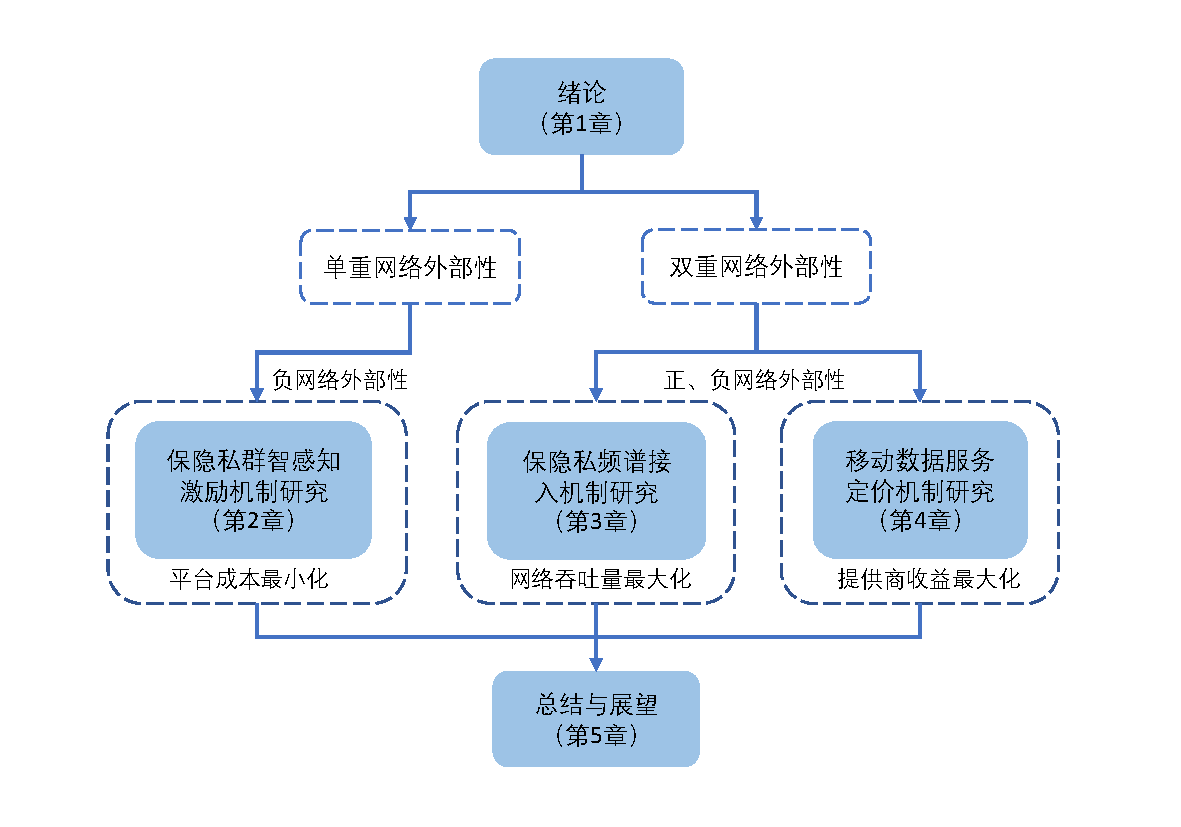
\includegraphics[width=1.05\textwidth]{pic/jiegou2.pdf}
\caption{全文组织结构图}
\label{fig:the}
\end{figure}

\subsection{研究内容}

本文的具体研究内容如下:

%毫米波通信系统中的多用户快速跟踪问题。由于毫米波通信与波束成形技术的引入,基站会通过很窄的波束与用户进行通信。精确的用户位置信息能够帮助更好地进行波束对准,因此基站需要准确地感知并估计小区内处于移动中的用户的个数及其各自位置信息,这就是一个多目标跟踪问题。同时,准确而快速的跟踪意味着更低的通信时延,因此毫米波通信中多目标跟踪的实时性也亟需提高。现有的高效多目标跟踪算法,如概率假设密度粒子滤波算法等,由于其中重采样算法的限制,难以做到流水线化计算,制约了实时性的进一步提高。本章提出一种改进的重采样算法,通过引入粒子复制序列集合以及待复制粒子序列,使得需要重采样的粒子在只获得自身信息与之前重采样粒子信息的时即可进行粒子复制运算,而不用等待所有粒子完成权重值过滤后才能继续重采样。通过引入此改进的重采样算法,整个概率假设密度粒子滤波算法能够实现完全流水线化的运算。在此基础上,本文提出基于多核处理器硬件平台的计算资源分配优化算法,通过解决一组混合整数规划问题,得到了高时效的近似解法。仿真结果验证了提出的算法在保证跟踪精度的情况下,能显著降低整个滤波算法的计算时延,有效地提高了用户跟踪的实时性,为基站中每个用户的低时延通信提供了保证。

%第3章研究了毫米波通信在星型网络拓扑下的典型应用——蜂窝小区网络中的资源优化问题。基站在已知小区内多个用户位置的情况下,优化分配资源以最大化系统收益即吞吐量。基站上的大规模天线阵列虚拟的分成若干个均匀线性子阵列,分别通过波束成形技术与对应的用户进行通信。由于大规模天线阵列与每个均匀线性子阵列都有着一定的固定的形状,因此问题建模为如何在矩形阵列中合理的放置这些子阵列,使得系统收益最大,这既需要考虑每个用户所占用子阵列的天线的数量,又需要考虑这些子阵列在矩形阵列中的位置分配。此场景根据不同的子阵列放置方式,又包含了两种不同的情况:1)所有线性子阵列都互相平行且平行于矩形阵列的一条边;2)为了进一步提高系统收益,线性子阵列可以平行于矩形阵列的任意一条边,即存在相互垂直的子阵列。对两种情况分别进行问题建模,对两个NP难问题进行分解并逐步求解。通过解决一系列的多选择背包问题,多背包问题和带状装箱问题,得到了两种情况下多项式时间的近似算法,并给出了每个算法的计算复杂度和下界。仿真结果验证了提出的两种算法在不同的情况下都能有效地分配天线资源,得到有性能保证的系统收益。

第二章考虑了数据隐私保护下群智感知系统平台成本最小化问题,提出了一种用于移动群智感知中隐私数据聚合的拍卖框架。由于移动用户的感知能力和提供数据的隐私成本皆有所差异,充当拍卖者角色的感知平台的主要挑战在于选择合适的参与用户,并针对性地为他们设计用于隐私保护的数据噪声分布,使得数据聚合结果达到准确性指标,同时用户的隐私得到保护并获取足够的奖励。本文提出了一种允许用户进行本地数据加噪的方案。其中用户所允许添加的噪声分布由感知平台决定,其数据隐私保护程度可以使用差分隐私的量化指标进行衡量。本文揭示了用户间所存在的{\kaishu 负网络外部性}效应,并根据用户对于隐私保护级别的偏好分成“消极隐私保护”和“积极隐私保护”两种场景进行问题的建模与求解。在“消极隐私保护”场景中当平台可以通过支付奖励充分补偿用户的隐私损失时,用户即愿意参与并提供感知数据。而在更具一般性的“积极隐私保护”场景中,参与用户对其数据隐私保护级别存在固有要求,仅当要求满足时才同意参与任务。基于问题隐藏的单调性特性,本文分别针对两种场景设计了具有诚实性、个体理性,计算效率高的激励机制,以近似地最小化感知平台用于购买用户数据的成本,同时满足对于聚合结果准确性的要求。我们通过理论分析结合充分的仿真实验验证了所提出的方案。

第三章考虑了位置隐私保护下具有社交意识的网络吞吐量最大化问题。在数据库辅助频谱共享的场景中,由于便携式移动设备与用户的强关联性,对移动设备的定位攻击给用户带来了位置隐私保护方面的担忧。本文中移动用户对信号传输功率水平添加随机扰动,以削弱基于RSS的潜在位置隐私攻击的威胁。另一方面,虽然用户之间的物理信号干扰({\kaishu 负网络外部性})会给网络整体性能带来负面影响,但用户之间社交关联引入的社交效应({\kaishu 正网络外部性})给系统效用带来了一定的提升空间。本文中,每个次级用户在进行频谱接入决策时,把包含其社交好友效用的“社交群体效用”作为自己的优化目标。进一步,本文将这种隐私保护下的具有社交意识的频谱共享问题建模成一个随机信道选择博弈。博弈中次级用户作为策略性的玩家动态调整其策略,以最大化其社交群体效用。我们针对博弈模型设计了一个基于无悔规则的双时间尺度分布式学习算法,并证明其几乎可以肯定收敛至博弈的相关均衡集合。数值结果证实,隐私保护级别越高,网络吞吐量的下降就越显着。

第四章考虑了服务提供商收益最大化问题。在竞争性数据服务市场中多个服务提供商通过定价策略的制定以最大化自身收益。市场中移动用户的数据消费行为同时受到两方面因素的影响:社交效应({\kaishu 正网络外部性})和拥塞效应({\kaishu 负网络外部性})。为了分析移动用户和服务提供商之间的策略互动,本文设计了一个两阶段的斯塔伯格博弈,分别由第一阶段的提供商博弈和第二阶段的用户博弈组成。针对用户博弈,本文刻画了均衡解的特征并建立了它的唯一性。对于提供商博弈,分析表明,对于提供商行为理性的场景以及提供商行为有限理性的场景,混合策略均衡解均是有保证的。进一步,本文提出了一种分布式学习算法,用于寻找提供商博弈的混合策略均衡解。最后,数值仿真结果对于正网络外部性和负网络外部性如何影响系统性能的提供了见解,并验证了提供商有限理性行为对其收益所产生的负面影响。

%第四章研究在毫米波通信在网状网络拓扑下的典型应用——无线数据中心网络中的资源优化问题。在下一代数据中心网络中利用毫米波高速无线传输代替传统服务器间有线连接,以提高数据中心网络灵活性及可扩展性等。随着数据流量特性的变化,网络中出现了流量极度不平衡现象,降低了整个网络的通信性能。数据中心的机房环境相对稳定,服务器间位置也相对密集且固定,因此可以通过60GHz毫米波无线通信建立服务器间点对点直接连接,减小通信热点带来的通信性能下降。设计在每个服务器机架顶(Top of Rack, ToR)布置毫米波天线,并提出适用于阵列天线的点对点视距通信六边形机架布置方案,同时建立了单层和三层的数据中心无线网络拓扑结构,提出了对应的网络节点与边生成方式。进而对建立的无线数据中心网络结构提出了天线资源优化分配问题,通过变量替换等方式将其转化为一几何规划问题进行求解。仿真结果验证了所提出毫米波无线数据中心网络结构与优化算法能够有效降低系统的最大通信时延。

最后,第六章对全文进行了总结,并提出了未来可能的研究方向。